\documentclass{article}

\usepackage[a4paper, total={7in, 9in}]{geometry}
\pagestyle{empty} % Prevent relative page numbers

%%%%%%%%%%%%%%%%%%%%%%%%%%%%%%%%%%%%%%
%% Default definitions 
%% Define listings format
\usepackage{xcolor} % Required for listings color definitions
\definecolor{Brown}{cmyk}{0,0.81,1,0.60}
\definecolor{OliveGreen}{cmyk}{0.64,0,0.95,0.40}
\definecolor{CadetBlue}{cmyk}{0.62,0.57,0.23,0}
\definecolor{lightlightgray}{gray}{0.9}

\usepackage{listings} % computer code language formatting

\lstdefinestyle{tex-style} {
	language=[LaTeX]TeX,                    % Code langugage
	basicstyle=\ttfamily,                   % Code font, Examples: \footnotesize, \ttfamily
	%keywordstyle=\color{OliveGreen},        % Keywords font ('*' = uppercase)
	commentstyle=\color{gray},              % Comments font
	numbers=none,                           % Line nums position
	numberstyle=\tiny,                      % Line-numbers fonts
	stepnumber=1,                           % Step between two line-numbers
	numbersep=5pt,                          % How far are line-numbers from code
	backgroundcolor=\color{lightlightgray}, % Choose background color
	frame=single,                             % A frame around the code
	tabsize=2,                              % Default tab size
	captionpos=b,                           % Caption-position = bottom
	breaklines=true,                        % Automatic line breaking?
	breakatwhitespace=false,                % Automatic breaks only at whitespace?
	showspaces=false,                       % Dont make spaces visible
	showtabs=false,                         % Dont make tabls visible
	columns=flexible,                       % Column format
	morekeywords={__global__, __device__}  % CUDA specific keywords
}
\lstnewenvironment{latex}
{\lstset{language=[LaTeX]TeX}}
{}
\lstset{style=tex-style}

%% Define URL format
\usepackage[hyphens]{url}
\usepackage{hyperref}
\hypersetup{
	colorlinks=true,
	citecolor=black,
	filecolor=black,
	linkcolor=blue,
	urlcolor=blue
}

\setlength\parindent{0pt}


%%%%%%%%%%%%%%%%%%%%%%%%%%%%%%%%%%%%%%
%% Example-specific packages
\usepackage{calc}
\usepackage{fp}
\usepackage{tikz}

%%%%%%%%%%%%%%%%%%%%%%%%%%%%%%%%%%%%%%
%% Example-specific preamble
\newlength{\mylength}
\newlength{\myotherlength}
\newlength{\templength}
%\newlength{\templength2} % Does not work, number is separated
\newcommand\FPuse[1]{\FPeval{\result}{#1}{\result}} % Used for direct calculations with fp. Manipulates the variable \result

\begin{document}

\section*{Calculations in LaTeX}

\subsection*{Description}
Programmatic execution and self-containment often require the performance of calculations within a \LaTeX document.
Two options dominate:

The \verb|calc| package is mostly intended for use in the manipulation of lengths. Be careful on the way it treats real numbers and the implicit unit conversion.

For more involved calculations, the \verb|fp| package provides a greater set of functionality.

Read the raw code for examples of broken code, in cases of syntactical omissions.

\subsection*{Sources}
\url{https://tex.stackexchange.com/questions/30081/how-can-i-sum-two-values-and-store-the-result-in-other-variable}\\
\url{https://ctan.org/pkg/fp}\\
\url{https://ctan.org/pkg/calc}

\subsection*{Used Packages}
\verb|calc, fp|

\subsection*{Preamble}
\begin{latex}
%%%%%%%%%%%%%%%%%%%%%%%%%%%%%%%%%%%%%%
%% Example-specific packages
\usepackage{calc}
\usepackage{fp}
\usepackage{tikz}

%%%%%%%%%%%%%%%%%%%%%%%%%%%%%%%%%%%%%%
%% Example-specific preamble
\newlength{\mylength}
\newlength{\myotherlength}
\newlength{\templength}
%\newlength{\templength2} % Does not work, number is separated
\newcommand\FPuse[1]{\FPeval{\result}{#1}{\result}} % Used for direct calculations with fp. Manipulates the variable \result
\end{latex}

\subsection*{Document}
\begin{latex}
	Length manipulation using the \verb|calc| package:
	
	\setlength{\mylength}{\textwidth}
	\setlength{\myotherlength}{3cm}
	
	\rule{\mylength}{5pt}
	
	\setlength{\templength}{\mylength-\myotherlength}
	\rule{\templength}{5pt}
	
	%\setlength{\templength}{\mylength-2*\myotherlength} % This doesn't work, because the untyped 2 will lated be assinged a unit type
	\setlength{\templength}{\mylength-\myotherlength*2}
	\rule{\templength}{5pt}
	
	\setlength{\templength}{\mylength-\myotherlength*\real{2.5}}
	\rule{\templength}{5pt}
	
	~\\
	The same commands work inside a tikz environment:\\
	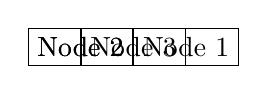
\begin{tikzpicture}
	\node[draw, anchor=west](n1) at (0,0) {Node 1};
	\node[draw, anchor=east](n2) at (\mylength,0) {Node 2};
	\draw (\mylength, 0) node[anchor=east] {Node 2};
	\setlength{\templength}{\mylength-\myotherlength*\real{2.5}}
	\node[draw](n3) at (\templength,0) {Node 3};
	\end{tikzpicture}
	
	~\\
	Arithmetic and algebra using \verb|fp| package:
	
	\FPset{varA}{10}
	varA = \varA
	
	\FPset{varB}{3}
	varB = \varB
	
	\FPeval{varC}{clip(varA+varB)}
	\varA + \varB = \varC
	
	\FPeval{varD}{round(varA^varB,3)}
	\varA \^\ \varB = \varD
	
	\FPmin{\varE}{\varA}{\varB}
	min(\varA, \varB) = \varE
	
	\FPlsolve{\varF}{\varA}{\varB}
	\varA*x+\varB=0 $\Rightarrow$ x=\FPuse{clip(\varF)}
	
	\FPeval{\varG}{arctan(\varA)}
	arctan(\varA) = \FPuse{round(\varG,3)}
	
	~\\
	The same functionality can be used within a math environment:
	\begin{equation}
	10\cdot x + 3 = 0 \Rightarrow x=\FPuse{clip(\varF)}
	\end{equation}
	
	~\\
	Sadly, the \verb|fp| package requires the full backslash notation (\textbackslash) to define variable names for several of its functions. This has the downside that numbers cannot be used as part of the variable name, as they cannot be included in a backslashed name.
\end{latex}

\subsection*{Result}
Length manipulation using the \verb|calc| package:

\setlength{\mylength}{\textwidth}
\setlength{\myotherlength}{3cm}

\rule{\mylength}{5pt}

\setlength{\templength}{\mylength-\myotherlength}
\rule{\templength}{5pt}

%\setlength{\templength}{\mylength-2*\myotherlength} % This doesn't work, because the untyped 2 will lated be assinged a unit type
\setlength{\templength}{\mylength-\myotherlength*2}
\rule{\templength}{5pt}

\setlength{\templength}{\mylength-\myotherlength*\real{2.5}}
\rule{\templength}{5pt}

~\\
The same commands work inside a tikz environment:\\
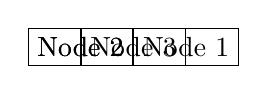
\begin{tikzpicture}
	\node[draw, anchor=west](n1) at (0,0) {Node 1};
	\node[draw, anchor=east](n2) at (\mylength,0) {Node 2};
	\draw (\mylength, 0) node[anchor=east] {Node 2};
	\setlength{\templength}{\mylength-\myotherlength*\real{2.5}}
	\node[draw](n3) at (\templength,0) {Node 3};
\end{tikzpicture}

~\\
Arithmetic and algebra using \verb|fp| package:

\FPset{varA}{10}
varA = \varA

\FPset{varB}{3}
varB = \varB

\FPeval{varC}{clip(varA+varB)}
\varA + \varB = \varC

\FPeval{varD}{round(varA^varB,3)}
\varA \^\ \varB = \varD

\FPmin{\varE}{\varA}{\varB}
min(\varA, \varB) = \varE

\FPlsolve{\varF}{\varA}{\varB}
\varA*x+\varB=0 $\Rightarrow$ x=\FPuse{clip(\varF)}

\FPeval{\varG}{arctan(\varA)}
arctan(\varA) = \FPuse{round(\varG,3)}

~\\
The same functionality can be used within a math environment:
\begin{equation}
10\cdot x + 3 = 0 \Rightarrow x=\FPuse{clip(\varF)}
\end{equation}

~\\
Sadly, the \verb|fp| package requires the full backslash notation (\textbackslash) to define variable names for several of its functions. This has the downside that numbers cannot be used as part of the variable name, as they cannot be included in a backslashed name.

\end{document}